\lecture{2}{21 Feb}{5-21}

\subsection{A service Description}

\begin{definition}[A service Description]\label{def:a_service_description_1}
    An infrastructure that provides services to applications.
\end{definition}

\begin{definition*}[Distributed applications]
    Applications involving multiple end systems that exchange data with each 
    other
    
    \begin{remark}[where they run]
        They run on end systems, they do not run in the packet switches in the 
        network core.
    \end{remark}
    
\end{definition*}


\begin{note}\label{note:postal_service_analogy_1}
    Alice wants to send a letter to bob.

    Alice needs to put th letter in an envelope, write Bob's details such as
    the address and the ZIP code, seal the envelope, put a stamp on it and 
    forward it to an official postal service.

    Similarly, the Internet employs a socket interface which must be adhered to 
    by the sending program for the Internet to route the data to the intended 
    receiving program.
\end{note}

\subsection{What Is a Protocol?}

\subsubsection{A human analogy}

\begin{figure}[h]
    \caption{Human analogy}
    \label{fig:human_analogy_1}
    \centering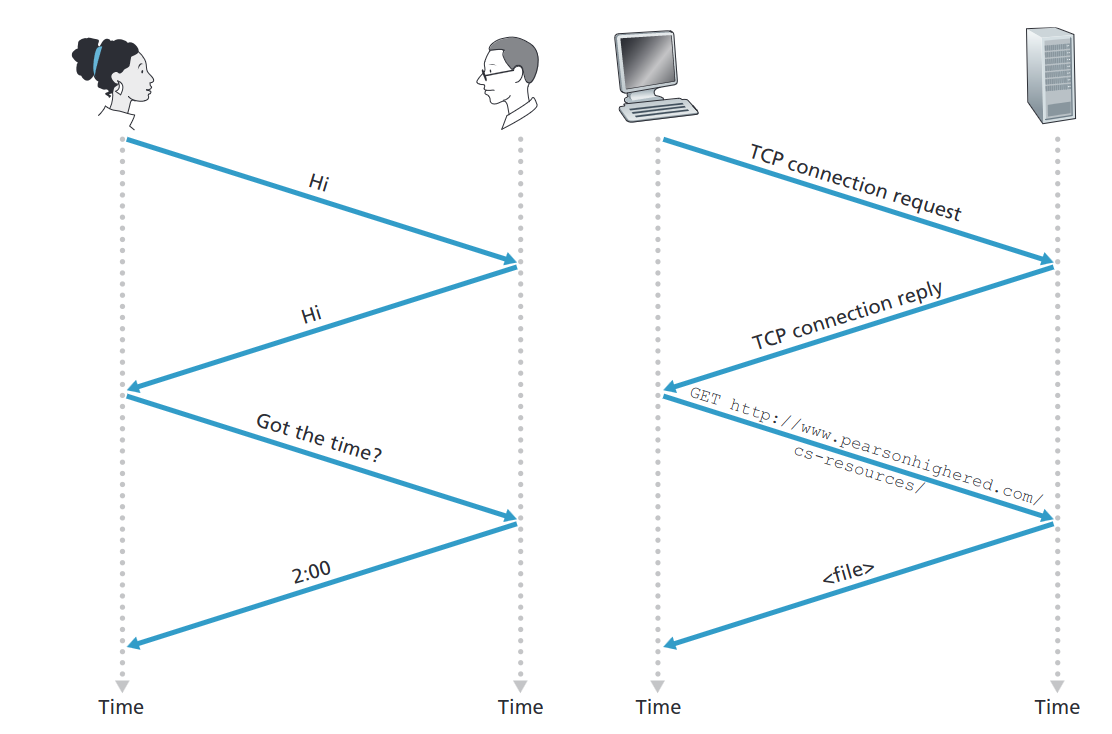
\includegraphics[width=0.5\textwidth]
    {Figures/lec_2_human_analogy.png}
\end{figure}



\newpage












